\documentclass[a4paper,12pt]{article} 
\usepackage[utf8x]{inputenc}
\usepackage[french]{babel}
\usepackage{mathtools}
\usepackage{amsmath, amssymb, amsfonts}
\usepackage{textcomp}
\usepackage[nointegrals]{wasysym}			% Collection de symboles mathématiques
\usepackage{ifthen}
\usepackage{tabularx}	 				% Gestion avancée des tableaux
\usepackage{longtable}		
%\usepackage{cleveref}

\usepackage{mathrsfs}

\usepackage{enumitem}
\usepackage{wrapfig}
%\usepackage[squaren]{SIunits}
%\usepackage[T1]{fontenc}				% Indispendable, présent dans tous les codes exemples
\usepackage[linkcolor=Indigo,colorlinks=true, citecolor=DarkSlateBlue, urlcolor=MidnightBlue]{hyperref} 	% Hyper ref
\usepackage{listings}					% Pour citer du code
\usepackage[justification=centering]{caption}
\usepackage{sistyle} 
\usepackage{numprint}
\usepackage{wrapfig}
\usepackage{cite}	
\usepackage{url} 					% Pour citer les sites internet dans la
%\usepackage{cleveref}
\usepackage{setspace}

\usepackage{graphicx}		 			% Inclusion des figures
\graphicspath{{./pic/}, {../figures/full_69_rapport/}}

\usepackage[svgnames]{xcolor}			%https://www.latextemplates.com/svgnames-colors


\usepackage{tikz} %Pour entourer un terme 
\newcommand*\circled[1]{\tikz[baseline=(char.base)]{
   \node[shape=circle,draw,inner sep=1pt] (char) {#1};}}
   
%%% Commandes utiles définies%
\newcommand{\argmin}{\mathop{\mathrm{argmin}}}

\newcommand{\bepar}[1]{
	\left( #1 \right)  
}

\newcommand{\becro}[1]{
	\left[ #1 \right]  
}

\newcommand{\beacc}[1]{
	\left\{ #1 \right \}  
}

\newcommand{\norm}[1]{
	\left \vert \left \vert #1 \right \vert  \right \vert
}

\newcommand{\rbk}[1]{\color{red}\textit{#1} \color{black}  
}

\usepackage{listings}					% Pour citer du code
%%%%%%%%%%%%%%%%%%%
%%% Élément pour citer des codes %%%
\lstset{
language=Python,
basicstyle=\ttfamily\bfseries\small, %
identifierstyle=\bfseries\color{black}, %
keywordstyle=\color{blue}, %
stringstyle=\color{black!90}, %
commentstyle=\it\color{black!70}, %
columns=flexible, %
tabsize=4, %
extendedchars=true, %
showspaces=false, %
showstringspaces=false, %
numberstyle=\small, %
breaklines=true, %
breakautoindent=true, %
captionpos=b,
otherkeywords={cross_val_score},
keywords=[0]{cv},
keywordstyle=[0]{\color{red}},
}
%%%%%%%%%%%%%%%%%%%%%
\title{\navy \textbf{Rapport CST fin première année} \color{black}}%%%%%%%%%%%%%%%%%%%%
\date{}
%\usepackage{multicol}
%\usepackage{etoolbox}
%\patchcmd{\thebibliography}{\section*{\refname}}
%    {\begin{multicols}{2}[\section*{\refname}]}{}{}
%\patchcmd{\endthebibliography}{\endlist}{\endlist\end{multicols}}{}{}
\usepackage[authoryear]{natbib}

\usepackage{geometry}
\geometry{hmargin=2cm, vmargin=1.8cm}

%%%%%%%%%%%%%%%%%%%%
%%% Couleurs %%%
\xdefinecolor{brick}{named}{DarkRed}
\xdefinecolor{navy}{named}{Navy}
\xdefinecolor{midblue}{named}{MidnightBlue}
\xdefinecolor{dsb}{named}{DarkSlateBlue}
\xdefinecolor{dgreen}{named}{DarkGreen}
\xdefinecolor{indian}{named}{IndianRed}

%%% 	Raccourcis 	%%%
\newcommand{\keps}{$k-\varepsilon$}
\newcommand{\covobs}{\text{C}^{-1}_{\text{obs}}}
\newcommand{\covpri}{\text{C}^{-1}_{\text{pri}}}
\newcommand{\bmap}{\beta_{\text{MAP}}}
\newcommand{\J}{\mathcal{J}}
\newcommand{\tinf}{$T_\infty$}
\newcommand\bk{\color{black}}
\newcommand\brick{\color{brick}}
\newcommand\navy{\color{navy}}
\newcommand\midblue{\color{midblue}}
\newcommand\dsb{\color{dsb}}
\newcommand{\dgreen}{\color{dgreen}}
\newcommand{\dpurple}{\color{indian}}
\newcommand\red{\color{red}}

%%%%%%%% Cigles
\newcommand{\rap}{par rapport}
\newcommand{\cad}{c'est-à-dire}
\newcommand{\vav}{vis-à-vis}
\newcommand{\NS}{Navier-Stokes}
\newcommand{\turb}{turbulence}
\newcommand{\inst}{instabilité}
\newcommand{\taur}{$\tau_{ij}$ }
%%%%%%%% Autres

%%%%%%%%%%%%%%%%%%%
% Syntax: \colorboxed[<color model>]{<color specification>}{<math formula>}
\newcommand*{\colorboxed}{}
\def\colorboxed#1#{%
  \colorboxedAux{#1}%
}
\newcommand*{\colorboxedAux}[3]{%
  % #1: optional argument for color model
  % #2: color specification
  % #3: formula
  \begingroup
    \colorlet{cb@saved}{.}%
    \color#1{#2}%
    \boxed{%
      \color{cb@saved}%
      #3%
    }%
  \endgroup
}

\renewcommand{\sectionmark}[1]{\markright{#1}}

\usepackage{fancyhdr}
\pagestyle{fancy}
\lhead{\textbf{Nathaniel} \brick \textbf{\textsc{Saura}}}
\rhead{\small Rapport première année}
%\rhead{\markright}
\cfoot{\thepage}
\renewcommand{\headrulewidth}{0.4pt}

\numberwithin{equation}{section} %%%% To count the equation like Section.Number

\usepackage{accents}
\newcommand{\vect}[1]{\accentset{\Rightarrow}{#1}}

\usepackage{multicol}		% Pour utiliser \hfill et découper une partie de son texte en colonnes
\setlength{\columnseprule}{0.pt}
%\def\columnseprulecolor{\color{red}}
%\setlength{\columnsep}{1.5cm}

% Numéro Roman pour le texte
\makeatletter
\newcommand*{\rom}[1]{\expandafter\@slowromancap\romannumeral #1@}
\makeatother

\begin{document}
\begin{titlepage} \centering
\vspace*{\fill}
\Huge \navy \textbf{Rapport CST fin première année} \bk \normalsize
\vspace*{\fill}
\end{titlepage}
%\maketitle
%\end{center}
\newpage

\navy \section{Introduction du sujet}  \bk
\Large{$\mathscr{L}$}\normalsize a turbulence est l'état d'un fluide dont l'écoulement possède des caractéristiques stochastiques, qui passionne les chercheurs et les ingénieurs depuis plusieurs siècles. %Même si Léonard De Vinci au $\overline{\underline{\text{XV}}}^{\, \text{ème}}$ siècle avait mentionné ce caractère aléatoire et décrit quantitativement le phénomène par des observations, Osborne Reynolds en 1883 amorça la description qualitative et mathématique que nous utilisons aujourd'hui; il fut suivi par d'autres grands noms de la mécanique des fluides comme Richardson, Kolmogorov puis d'autres. \\
%Il construisit le nombre caractéristique dit de Reynolds qui compare les effets d'inertie et les effets visqueux. \\
%\noindent Cette discipline est une des branches de la mécanique des fluides les plus actives qui attire énormément de chercheurs d'horizons plus ou moins éloignés de la mécanique des fluides. \\ %Kolmogorov sus-mentionné était avant tout mathématicien.\\
%Il existe de nombreux facteurs qui jouent sur la popularité de la discipline, sans être exhaustif, il est possible d'en développer deux : dans un premier temps cette théorie traite d'écoulement que l'on retrouve autour de soi dans notre vie de tous les jours (sillage d'une voiture, couche limite sur les ailes d'un avion etc...) mais également dans les océans, le ciel et l'espace. \\
%Le deuxième facteur clé découle du premier : au fur et à mesure que de nouvelles technologies impliquant ce genre d'écoulement émergent, de l'intelligence provenant d'autres domaines de la Physique, de l'Informatique ou des Mathématiques devient nécessaire voire indispensable. \\
Au travers de ses équations, la théorie de la Turbulence entend modéliser les fluides dont les effets d'inerties ne sont pas négligeables devant les effets visqueux. Les équations de Navier-Stokes constituent la base de cette discipline. Si on considère une parcelle de fluide et que l'on y effectue un bilan de quantité de mouvement, on obtient dans un cas incompressible \footnote{Sans forces extérieures, avec $\rho$ la masse volumique (constante), $\nu$ la viscosité cinématique de l'écoulement et $p$  le champ de pression} :\\
\begin{equation}
\frac{\partial u_i}{\partial t} + \underset{\text{\red Inertie -  terme non linéaire \bk}}{\text{\red \circled{\bk $u_j\, \frac{\partial u_i}{\partial x_j}$}}} \bk = - \frac{1}{\rho} \frac{\partial p_i}{\partial x_j} + \underset{\text{\navy Visqueux \bk}}{\text{\navy \circled{\bk $\nu \frac{\partial^2 u_i }{\partial x_j^2}$}}} \bk 
%\tag{Navier-Stokes} 
\end{equation}
Les termes d'inerties ou de convection (nous considérons ici des flux ou des transports d'énergie mesurés en Watt) apparaissent dans le terme non-linéaire des équations de Navier-Stokes traduisant l'apport local d'énergie cinétique du fluide autour de la parcelle contrôlée. La viscosité d'un fluide traduit sa capacité à dissiper l'énergie de l'écoulement sous forme de chaleur.\\

Reynolds construisit un nombre sans dimension comparant les effets d'inertie sur les 
effets visqueux; il est appelé nombre de Reynolds, abrégé Reynolds; il peut s'écrire comme $$ \text{Re} = \bepar{u_j\, \frac{\partial u_i}{\partial x_j}} / \bepar{\nu \frac{\partial^2 u_i }{\partial x_j^2}} = \frac{\text{Effets inertiels} }{\text{Effets visqueux}} $$ 
Ce nombre  caractérise l'état de l'écoulement. Pour un Reynolds faible (jusqu'à quelques centaines voire quelques miliers selon les cas), l'écoulement est dit laminaire. Lorsqu'il est au delà de la dizaine de milliers, l'écoulement est dit turbulent. \\
Entre les deux états, on parlera d'état de transition : des instabilités naissent dans l'écoulement rendant le champ de vitesse fluctuant. Plus le Reynolds augmente et plus ces fluctutations sont fortes, jusqu'à arriver à un champ de vitesse complétement aléatoire (turbulent). \\

\noindent  Par analyse dimensionnelle, le nombre de Reynolds peut être construit comme le rapport 
\begin{equation}
 \text{Re} = \frac{\text{UL}}{\nu}
\end{equation} 
 La notion clé dans la théorie de la turbulence est que les échelles spatiales L, temporelles T et leurs combinaisons (comme la vitesse U = L/T) se décomposent en un nombre très élevé de sous-échelles.
Dans le cadre de la turbulence, on fera allusion au Reynolds des plus grandes échelles lorsqu'il sera question de nombre de Reynolds sans plus de précision sur l'échelle spatiale ou de vitesse. \\
Le passage du laminaire au turbulent est marqué par un changement topographique de l'écoulement. La première structure turbulente qui apparaît est en général un tourbillon dont les échelles caractéristiques sont similaires à celles du Reynolds «global». Sur ces échelles on pourra définir un temps caractéristique de retournement du tourbillon $\tau_{\text{retournement}} = L/U$. \\
Plus le Reynolds est grand et moins le fluide sera capable d'absorber les instabilités induites par l'inertie du fluide. En conséquence, à haut Reynolds, de l'énergie est constamment injectée dans la zone d'intérêt. Cette énergie est à l'origine de la multitude des échelles spatiales (et donc de toutes les autres) ; on parle de cascade\footnote{L'idée de cascade fut proposée par Richardson, mais sa description s'est avérée fausse. Kolmogorov en 1941 mis en évidence la casacade de Richardson de manière plus mathématique, sans pour autant utiliser cette appellation.} ou de brisure des échelles, \cad $ $ que l'énergie cinétique des premières structures de turbulence est distribuée à des structures de taille plus petite. Ce processus est répété jusqu'à ce que le fluide soit capable de dissiper en chaleur l'énergie cinétique liées aux structures ainsi créées. \\

\noindent D'un point de vue pratique, les équations de \NS $ $ ne sont actuellement solubles «à la main» seulement pour des cas relativemenent simples. Pour la majorité des écoulements turbulents, il est nécessaire d'utiliser des outils numériques.\\
L'approche la plus précise pour résoudre ces équations est la méthode dite directe, ou DNS (Direct Numerical Simulation). Cette méthode entend résoudre les équations de \NS $ $ à toutes les échelles, et nécessite donc un maillage très resserré dans toutes les dimensions du problème, dont le pas est donnée par la théorie elle même. \\
La DNS nécessite des ordinateurs très performants et souvent plusieurs mois de calculs. Ces résultats sont utilisés comme référence (au même titre que les résultats expérimentaux) et de base pour évaluer les résultats de modèles numériques moins couteux et moins précis.\\
Dans un ordre de précision, les méthodes dites de LES (Large Eddy Scales) suivent les DNS. Schématiquement, cette catégorie de méthodes consiste à définir un seuil de prise en compte des échelles, accélérant ainsi les calculs. Pour assurer une prise en compte de la physique des plus petites échelles, différents termes modélisant l'action des petite échelles et leurs avec les plus grandes sont construits. Ces méthodes sont fiables mais encore trop lentes pour un usage en industrie.\\

\noindent Enfin, il existe une dernière catégorie appelées RANS qui regroupe des méthodes rapides mais dont la fiabilité varie fortement selon les cas. Les designers de ces approches entendaient résoudre la turbulence uniquement pour les grandes échelles. La modélisation des échelles plus petites se fait par l'ajout d'équation(s) de transport (comme Navier-Stokes) pour des grandeurs clés de la turbulence comme l'énergie cinétique turbulente $k$, du taux de dissipation de cette énergie $\varepsilon$, parfois les deux, ou d'autres quantités. On parle de modèle à un ou deux équations. \\% (comme l'intermittence $\gamma$ ou la viscosité turbulente $\nu_T$).\\
%; les plus connus sont le \keps, le Spalart-Allmaras et le $k-\omega$.\\

\noindent Les grandes échelles évoquées ici correspondent en fait au champ moyen de l'écoulement. En effet, une des idées de base de la théorie de la turbulence est la décomposition, dite de Reynolds. Elle consiste à écrire un champ turbulent en une somme d'une partie moyenne (temporelle) et d'une partie fluctuante. Les conventions variant d'un auteur à l'autre, dans le cadre de ce travail, les champs moyens seront écrits avec une barre au dessus (par exemple $\overline{U_i}$), les champs fluctuants seront écrits en minuscule. \\
Lorsque l'on injecte cette décomposition dans les équations de \NS $ $ sur la vitesse et la pression, on peut distinguer deux équations, une pour chacun des champs moyen et fluctuant. Pour plus de clarté, on écrit l'équation de \NS $ $ pour le champ moyen : 
\begin{equation}
 \frac{\partial \overline{U}_i}{\partial t} + \overline{U}_j \frac{\partial \overline{U}_i}{\partial x_j} = -\frac{1}{\rho} \frac{\partial \overline{P}}{\partial x_j} + \nu \frac{\partial^2 \overline{U}_i}{\partial x_j^2}  - \frac{\partial \, \overline{u_iu_j}}{\partial x_j} \label{meanfield}
 \end{equation}
  Cette équation est appelée RANS pour Reynolds Averaged \NS. On peut remarquer que l'évolution du champ moyen prend en compte des quantités moyennes mais aussi un flux d'énergie cinétique de la partie fluctuante. Ce flux d'énergie représentée par le tenseur d'ordre deux $-\rho \overline{u_iu_j}$ est appelé tenseur de Reynolds. On le note $\tau_{ij}$.\\
Pour modéliser $\tau_{ij}$, il est nécesaire de modéliser le tenseur d'ordre trois $-\overline{u_iu_ju_k}$ dont la modélisation nécessite celle du tenseur d'ordre quatre $-\overline{u_iu_ju_ku_l}$ et ainsi de suite. \\
%Le fait de d'avoir besoin d'un tenseur d'ordre n+1 pour la modélisation de celui d'ordre n schématise la cascade sus-décrite et indique que les fluctuations aux différentes échelles sont fortement couplées.\\
  Il s'avère en fait que le système formé des équations RANS et de celles du champ fluctuant est ouvert \cad $ $ qu'il y a plus d'inconnus que d'équations, il faudra rajouter une équation de fermeture, c'est l'objet des méthodes à une ou plusieurs équation(s).\\ %L'effort dans ces approches et de simuler le terme de fluctuations pour obtenir le champ moyen, d'où l'appellation RANS.\\
  
\noindent Dans ces méthodes RANS, on utilise l'hypothèse de Boussinesq. Celle-ci se base sur le fait que la création de nouvelles échelles augmente la stochasticité du champ de vitesse et donc de la friction au sein de l'écoulement.\\
  Il est alors proposé de construire un terme de viscosité liée à la turbulence à partir d'une analagie à la viscosité cinématique. La formule proposée par Boussinesq en 1890 s'écrit alors : 
\begin{equation}
\tau_{ij} = \rho \nu_T\bepar{\frac{\partial \overline{U}_i}{\partial x_j} + \frac{\partial \overline{U}_j}{\partial x_i}} - \frac{2}{3} \rho \overline{u_iu_i} \delta_{ij} \label{boussi}
\end{equation} 
La troisième et dernière idée des méthodes RANS est d'utiliser des observations pour écrire des relations entre différentes quantités turbulente de l'écoulement, en s'appuyant également sur \eqref{boussi}. \\
Par exemple pour les modèles à deux équations \keps $ $ ou $k-\omega$ respectivement, on utilisera une relation entre $k$ $\nu_t$ et $\varepsilon$ (resp. $\omega$). Les équations de transports modéliseront l'évolution (spatiale car ce sont des modèles stationnaires) de $k$ et de $\varepsilon$ (resp. $\omega$). Ces équations sont construites en injectant des constantes empiriques qui ont pour but de modéliser les actions (et les rétro-actions puisqu'il y a couplage) des petites échelles.\\

%Pour les approches DNS les résultats corroborent exactement avec les résultats expérimentaux, la majeur contrepartie est le temps de calculs qui est encore très élevé malgré la parallélisation massive et l'utilisation de cluster d'ordinateurs. \\
%Pour les méthodes LES et RANS les modélisations des effets de petites échelles ont tendance à perturber les résultats et impliquent une perte de précision. En revanche, pour des écoulements complexes les résultats sont bien plus probants avec l'approche LES que l'approche RANS.\\
%Les méthodes RANS reposent beaucoup sur des constantes dont les valeurs sont déterminées par l'intuition, du réglages ou sur des valeurs standards définies à partir d'observations expérimentales sur une plage de cas peu variés, ou du moins non représentatif de la variété et la complexité des écoulements que l'on peut retrouver dans la nature.\\
%Alors que les industriels n'utilisent en majorité que ce type d'approche afin de générer des résultats représentatifs rapidement, la question de la fiabilité des résultats se pose. En parallèle la théorie de la turbulence n'a que très peu avancé depuis les années 1980 et de nouvelles approches doivent être explorées comme il fut fait dans le passé.\\[2mm]

\noindent Au fur et à mesure que les méthodes numériques se développaient, les machines et les méthodes expérimentales se perfectionnaient, une quantité importante de données a pu être accumulée couvrant des écoulements classiques aux complexes, balayant des topologies variées et des spécificités propres aux différentes branches de la mécanique des fluides. Des méthodes ayant pour but d'utiliser ces données ont alors vu le jour, on parle de méthodes pilotées par les données. Une des plus couramment utilisée est la méthode dite d'inversion : elle consiste à retrouver les paramètres d'un modèle, disposant auparavant des données issues de ce dernier et de ses variables d'états. \\

\noindent En parallèle, une forme de méthode pilotée par les données vit également le jour dans les années 1950 ce sont les intelligences artificielles : des algorithmes capable de découvrir une règle implicite dans les données liant les caractéristiques avec les observations, les entrées et les sorties. En plus d'«apprendre» ces règles, ces algorithmes sont capables de prédire la sortie d'entrées inédites, \cad $ $ de généraliser leur apprentissage. \\
Ces méthodes ont connu une explosion dès lors que les ordinateurs ont gagné en puissance et en capacité. Depuis les années 2000, la recherche en Physique a vu l'incorporation toujours plus grande d'IA que ce soit pour améliorer la prédiction de modèles plus ou moins fiables, pour l'analyse de données, pour la détection de structures entre autres. \\

\noindent Un des objectifs de notre thèse est d'utiliser les intelligences artificielles et les méthodes pilotées par les données pour améliorer les résultats de modèles peu fiables comme le RANS, mais également fournir d'autres outils de prédictions, en s'assurant que la Physique au travers les lois de conservation, est bien respectée.

%\noindent 
%Le procédé est le suivant : on injecte un terme optimisable dans les équations du modèles le moins précis, on évalue en chaque point la différence entre la solution fournie par ce dernier et la solution attendue (celle de référence), puis grâce à des méthodes d'opimisation on s'assure que le terme injecté corrige suffisamment bien cet écart jusqu'à atteindre le seuil voulu. \\
%Ce procédé s'appelle la «maximalisation \textit{a posteriori}» de la fonction évaluant la probabilité d'obtenir le bon terme correctif sachant les observations disponibles.
%Ainsi théoriquement, il devient possible de combiner rapidité de calcul et précision en «augmentant» les modèles RANS ou LES avec un terme correctif issu des données.\\
%Cependant, cette inversion reste limitée par l'existence et la disponibilité de telles données, ce qui empêche la généralisation de cette même méthode.\\

%La solution à ce problème fut également élaborée le siècle dernier. En effet, des méthodes d'apprentissage et de généralisation de pattern émergèrent. Une fois encore, la communauté scientifique saisit l'énorme (voire infini) potentiel de ces algorithmes avec l'amélioration des capacités des ordinateurs et la disponibilité des données.\\ L'ensemble de ces méthodes sont désignées aujourd'hui sous l'appellation d'intelligence artificielle (IA). Bien implémentées, ces méthodes permettent d'assimiler le processus liant les données entre elles et permettent sous certaines conditions de généraliser les données.\\

\noindent Avant d'entrer dans le vif du rapport, nous en présentons succintement le plan : le cœur de la première partie sera l'inférence et sa généralisation par réseau de neurones ou autres algorithmes. Les étapes du procédés seront détaillées ainsi que des résultats obtenu sur des problèmes différents. Les objectifs sur le court et le moyen terme seront également évoqués.\\
La deuxième partie se concentrera sur l'utilisation des réseaux de neurones comme seul outil de prédiction. Plusieurs remarques concernant le devenir de ces travaux au cours des deux prochaines années seront faites.\\
Dans une troisième partie plusieurs pistes d'études autour de ces thématiques seront abordées de manières plus brèves. L'accent sera porté sur l'origine de ces idées et sur l'importance qu'elles occuperont par la suite.

\pagebreak

\navy \section{Combiner vitesse et précision au travers l'association inférence et machine learning} \label{combiNN_inference}
 \bk
\noindent L'élaboration d'une théorie Physique ainsi que sa vérification sont toujours pilotées par les données. En effet, face à une situation (un écoulement, une onde se propageant...), les scientifiques réalisent des mesures des quantités d'intérêts, essaient de déterminer les variables décrivant le phénomène et établissent des équations liant ces variables et les quantités observées. Ils confrontent ensuite leur théorie avec les mesures réalisées en amont. \\
Si la correspondance est bonne, la théorie est acceptée et testée dans d'autres cas. Si les équations ne rendent pas compte convenablement de la réalité, elles sont retravaillées. \\
Cette procédure résume les différentes étapes de l'inférence Bayesienne dans la recherche de paramètres optimaux alliant prédictions et observations.
 
 
\brick \subsection{Présentation de l'inférence et de ses outils} \bk
\noindent L'inférence ou l'inversion consiste à résoudre un problème de la solution aux entrées. \cad $ $ qu'à partir d'observations et d'équations présentant des paramètres notés dans un vecteur $\beta$, réaliser une inversion consiste trouver les valeurs des composantes de ce vecteurs de paramètres, minimisant le plus possible l'écart entre la solution observée et celle obtenue avec les équations paramétrées. \\
Nous proposons ici de rentrer plus en détail dans la théorie et dans son utilisation.

\dsb \subsubsection{Théorème de Bayes et fonction de correspondance} \bk
\noindent L'inférence Bayesienne se base sur le théorème de Bayes établit fin du $\overline{\underline{\text{XVIII}}}^{\, \text{ème}}$ siècle. Il permet d'évaluer une distribution de probabilité des paramètres que l'on cherche à évaluer, sachant les observations ou les mesures.\\
Dans l'étude présentée, le paramètre recherché est un vecteur noté $\beta$. Le théorème de Bayes permettra d'évaluer la probabilité $p\bepar{\beta\,|\,\textbf{d}}$, \textbf{d} représentant les observations; il établit 
\begin{equation}
p\bepar{\beta\,|\,\textbf{d}} = \frac{\mathcal{L}\bepar{\textbf{d}\,|\,\beta}p\bepar{\beta}}{c} %\tag{Théorème de Bayes}
\end{equation}
Ce théorème lie la distribution de correspondance ou \textit{likelihood distribution} $\mathcal{L}\bepar{\textbf{d}\,|\,\beta}$, avec la distribution \textit{a priori} $p\bepar{\beta}$, du vecteur $\beta$. $\mathcal{L}$ représente la probabilité d'obtenir les observations sachant un premier essai de $\beta$ (on parlera d'information \textit{à priori}),\\
Au dénominateur, le terme $c$ représente la \textit{likelihood marginalisée} par tous les paramètres possibles. Le but étant de construire une moyenne de $\mathcal{L}\bepar{\textbf{d}\,|\,\beta}$ par rapport aux choix de paramètres à priori. $c$ s'écrira donc 
\begin{equation}
c = \int_{\beta} \mathcal{L}\bepar{\textbf{d}\,|\,\beta}p\bepar{\beta} d\beta
\end{equation} \\
Calculer $p\bepar{\beta\,|\,\textbf{d}}$ peut se faire en supposant que \textbf{d}, $\beta$ et $\mathcal{L}$ ont des distributions gaussiennes comme suggéré par \citep{parish2016paradigm}, \citep{tarantola2005inverse} ou d'autre.\\
La méthode MAP pour \textit{Maximum A Posteriori} utilisée par les références citées, consiste à calculer la valeur de $\beta$ la plus probable plutôt que de déterminer de l'entière distribution. L'objectif est alors de maximiser la correspondance entre modèle et observation soit 
\begin{equation}
\beta_{\text{MAP}} = \underset{\beta}{\text{arg}\, \text{max}} \ p\bepar{\beta\,|\,\textbf{d}} \label{bmap}
\end{equation}

\noindent À partir de développement mathématiques dont il ne sera pas question ici, il est possible d'écrire $\mathcal{L}$ comme une fonction de coût.\\
Souvent les données expérimentales sont obtenues avec une incertitude propre à la méthode de mesure ou aux outils utilisés. Ces incertitudes devant apparaître, on construit une matrice de covariance $\covobs$ (nous n'utiliserons que son inverse). \\
Idem, puisque $\mathcal{L}$ prend en compte la première valeur (premier choix ou first guess) $\beta_{\text{pri}}$ et sa distribution, la fonction de coût équivalente doit faire apparaître la covariance $\covpri$.\\
Finalement avec $\textbf{h}_\beta \equiv \textbf{h}(\beta)$ la prédiction du modèle qu'on essaie de corriger, effectuer une inversion revient à estimer 
\begin{equation}
\bmap = \underset{\beta}{\text{arg}\, \text{min}}\ \frac{1}{2}\becro{\bepar{\textbf{d} - \textbf{h}_\beta}^T \covobs \bepar{\textbf{d} - \textbf{h}_\beta} + \bepar{\beta - \beta_{\text{pri}}}^T \covpri  \bepar{\beta - \beta_{\text{pri}}}} \label{bmapJ}
\end{equation}
La fonction à minimiser est la fonction de coût sus-mentionnée, elle est notée $\mathcal{J}$ dans la suite.

\dsb \subsubsection{L'algorithme BFGS} \bk

\noindent La résolution de ce problème devient alors un problème de minimisation. Nous utilisons l'algorithme Broyden-Fletcher-Goldfarb-Shanno abbrégé BFGS dans la suite \citep{nocedal2006numerical}.
Contrairement aux Algorithmes de gradient classiques, le BFGS est un algorithme d'ordre deux. Il utilise une une approximation de la hessienne de $\J$ afin de ne pas avoir à effectuer le calcul de cette matrice qui peut s'avérer très lourd.\\
C'est une méthode itérative mettant à jour le vecteur d'intérêt $\beta_k$ ainsi que sa hesienne inverse notée $B^{-1}_k$ à partir d'un algorithme d'exploration appelé \textit{line search} dont nous évoquerons brièvement les spécificités.\\
Pour atteindre le minimum global de l'équation \eqref{bmapJ}, il est nécessaire d'incrémenter la valeur de $\beta_k$ par une variation $d\beta_k$ vérifiant l'inégalité suivante
\begin{equation}
\nabla\J_k = \frac{\partial \J}{\partial \beta_k} = \frac{\J\bepar{\beta_k+ d\beta_k} - \J\bepar{\beta_k}}{d\beta_k} < 0
\end{equation}
Pour déterminer la forme de cet incrément le BFGS procède en deux étapes : dans un premier temps l'algorithme détermine la \textit{direction} du gradient puis la \textit{longueur} de l'incrément. \\
On note le vecteur de direction $\mathbf{p}_k$, il s'écrit :
\begin{equation}
\mathbf{p}_k = -B_k^{-1}\nabla_k\J
\end{equation}
Pour vérifier que ce vecteur pointe dans la bonne direction, le produit scalaire du gradient $\nabla_k\J$ projeté sur la hessienne doit vérifier l'inéquation:
\begin{equation}
-\nabla_k^T\J\, B_k^{-1}\, \nabla_k\J = \mathbf{p}_k^T\, \nabla_k\J < 0
\end{equation}
Cette condition est une conséquence directe du développement de Taylor autour de l'incrément.\\

\noindent Une fois la direction calculée, il reste à déterminer l'amplitude de l'incrémentation. En effet, puisque l'on cherche le minimum global de $\J$, il faut veiller à ne pas «tourner autour» du $\bmap$ indéfiniment, et adapter le pas au fur et à mesure que l'optimisation se déroule.\\ 
Sans rentrer dans dans tous les détails, le BFGS utilise un algorithme de \textit{line search} pour trouver $ \displaystyle \alpha_k$ tel que $d\beta_k = \alpha_k\mathbf{p}_k$. Cette recherche doit satisfaire deux critères sur $\beta_{k+1}$: 
\begin{itemize}
\item[$\bullet$] Une condition sur la nouvelle valeur de la fonction de coût : \begin{equation}
\J\bepar{\beta_{k+1}} - \J\bepar{\beta_k} < C_1
\end{equation} 

\item[$\bullet$] Une condition sur la pente (ou la courbure) : 
\begin{equation}
|\nabla\J \bepar{\beta_{k+1}}^T\textbf{p}_k| < C_2 |\nabla\J \bepar{\beta_k}^T\textbf{p}_k|
\end{equation}
\end{itemize} 
$C_1$ et $C_2$ étant deux seuils préalablement définis.\\
La dernière étape de l'algorithme consiste à incrémenter $B_{k+1}^{-1}$ utilisant $\alpha_k$ ainsi que d'autres termes construit à partir de $\beta_{k+1}$.\\

\pagebreak

\brick \subsection{Utilisation de l'inférence sur différents cas} \bk

\noindent Nous avons mis en place les outils présentés ci-dessus dans plusieurs cas, nous n'en présenterons que deux : un problème thermique monodimensionnel provenant de \citep{parish2016paradigm}, puis sur la propagation d'une onde à travers l'équation de Burgers 1d. \\
Nous travaillons également sur l'utilisation de ce procédé pour trouver les paramètres  qui corrigeraient les modèles le moins précis (par exemple RANS ou LES) réduisant alors l'écart les solutions références(DNS ou expériences).

\dsb \subsubsection{Problème thermique} \bk
Le but est d'établir l'évolution du champ de température dans un barreau dont les températures au début et en fin de domaine sont nulles. Cette évolution se fait sous des termes de conduction, de convection et de radiation. Le paramètre de ce problème sera la température extérieure au barreau $T_\text{inf}$. 
L'équation exacte qui régit ce problème s'écrit 
\begin{equation}
 \frac{d^2T}{dz^2} + \varepsilon(T)\bepar{T^4_\infty - T^4} + h\bepar{T_\infty - T} = 0 \label{Ttrue} \tag{EE}
 \end{equation} 
 Avec 
 \begin{equation}
 \varepsilon(T) = \becro{1 + 5 \sin\bepar{\frac{3\pi}{200}\, T} + \exp\bepar{0.02\,T}+ \mathcal{N}\bepar{0,\, 0.1^2}} \times 10^{-4} \label{epsilon}
 \end{equation}
 On commence par résoudre ce problème exact pour plusieurs tirage de $\varepsilon$. On utilise la méthode de Crank-Nicholson pour résoudre ce problème, en ajoutant artificiellement un terme d'évolution temporelle $\displaystyle \frac{dT}{dt}$.\\
 En même temps de construire une dataset de référence, on évalue la sensibilité des résultats par rapport à la distribution $\mathcal{N}$ présente dans l'équation \eqref{epsilon}. Cette sensibilité se traduit par la construction d'une matrice de covariance des données observables issues de ce problème exact.\\
 Afin de tester l'inférence, nous biaisons l'équation exact \eqref{Ttrue} pour obtenir (E$\beta$) :
\begin{equation}
\frac{d^2T}{dz^2} + \varepsilon_0\beta(z)\bepar{T^4_\infty - T^4}= 0 \tag{E$\beta$} \label{Tinex}
\end{equation}
Nous construisons $\covpri$ en diagonalisant des valeurs fournies par \citep{parish2016paradigm}.\\

\noindent Au cours de la minimisation,  afin de pouvoir voir la solution se dessiner, il a été nécessaire de coder un solver BFGS en suivant \citep{nocedal2006numerical}. Un exemple de cette évolution pour \tinf = $50$ est illustrée Fig.\eqref{tinf50cpt_500}.\\
Le critère de convergence est ici une condition sur $||\nabla_{\beta_k}\J||_\infty$ ou bien sur un nombre limite d'itérations. La figure Fig.\eqref{evolT50} récapitule l'évolution de cette grandeur en cours d'optimisation.\\

\noindent La méthode BFGS permet également d'avoir accès à la hessienne inverse de $\J$ évaluée sur $\bmap$. Grâce à sa décomposition de Cholesky, on peut construire une approximation de la distribution $p\bepar{\beta\,|\,\textbf{d}}$ autour de $\bmap$. 
On note $R$ tel que $\text{Chol}\bepar{B_{\bmap}^{-1}} = \text{R}\text{R}^T$ et $s \sim \mathcal{N}\bepar{0,1}$. Ainsi 
\begin{equation}
p\bepar{\beta\,|\,\textbf{d}} \approx \bmap + \text{R}s \label{distribbmap}
\end{equation}
Il devient possible d'évaluer la variance de cette distribution. Sur 250 tirages de $\beta$, on résout \eqref{Tinex}, on calcule les extrema ainsi que les déviations standards. On fait de même avec $\bmap$ solution de l'optimisation de Scipy, et l'on compare les extrema sur chacun des points du domaine; disposant d'une écriture analytique pour $\beta_{\text{True}}$, on peut évaluer la fiabilité de la méthode en traçant toutes ces grandeurs dans une même figure voir Fig.\eqref{comp_bmap_hbmap}. \\
 Il arrive que la méthode scipy sorte de la boucle d'optimisation pour des raisons propres à l'implémentation. C'est en parti pour cela que nous avons recodé la méthode, et aussi pour comprendre le processus et avoir accès aux différents $\beta$, aux valeurs des hessiennes inverse etc.\\
 Le temps de calcul est toutefois nettement plus conséquent avec le code «maison». Les différences ne sont jamais vraiment grandes à part pour le cas \tinf = 50 que nous présentons ici. 

\begin{figure}[!ht]
\centering
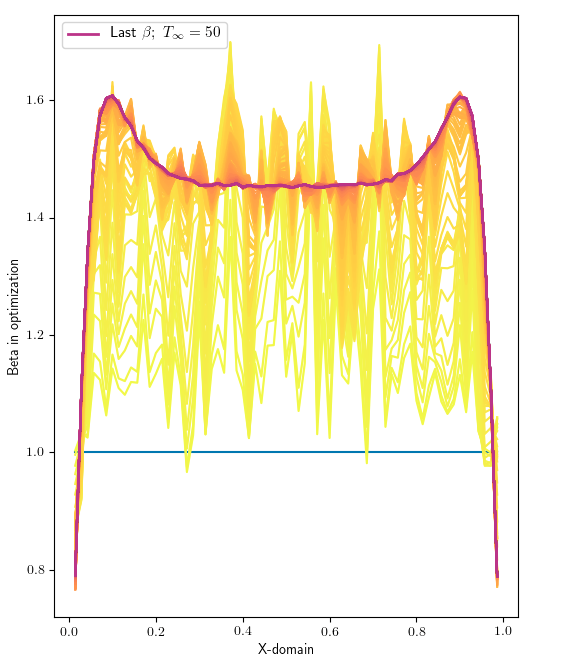
\includegraphics[width=9.7cm, height=11cm]{Just_bmapTinf50.png}
\caption{\small{À gauche évolution de beta au cours de l'optimisation pour $T_\infty$. La droite bleue représente le first guess de $\beta$. Plus la teinte est foncée plus on se rapproche de $\bmap$.}}
\label{tinf50cpt_500}
\end{figure}

\begin{figure}[!ht]
\centering
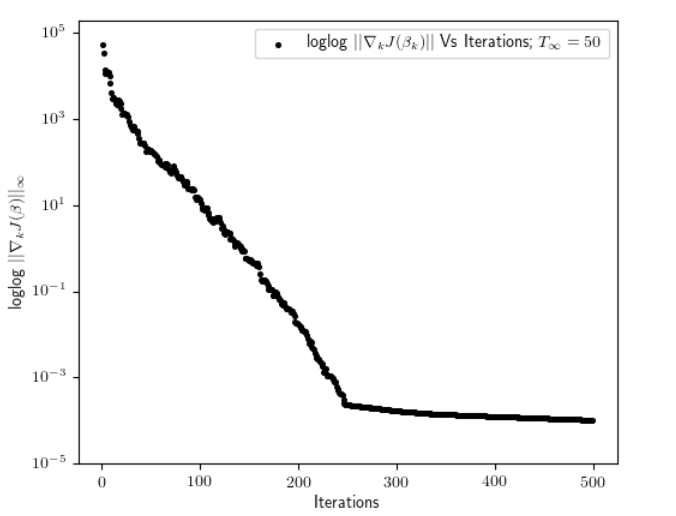
\includegraphics[scale=0.75]{bmap_adjbfgs_T50500png.png}
\caption{\small{Évolution de la norme infinie du gradient de la fonction de coût évalué en $\beta$ au cours de l'optimisation. On voit que cette grandeur tend vers une valeur bien inférieure à zéro, attestant la convergence de l'optimisation.}}
\label{evolT50}
\end{figure}

\begin{figure}[!ht]
\centering
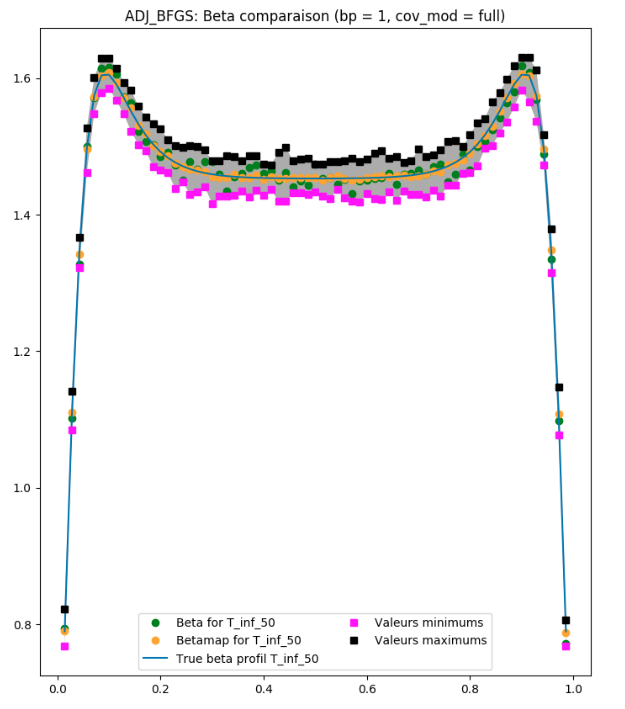
\includegraphics[height=10cm, width=8.43cm]{bmap_50_adjVStheo.png} \hfill
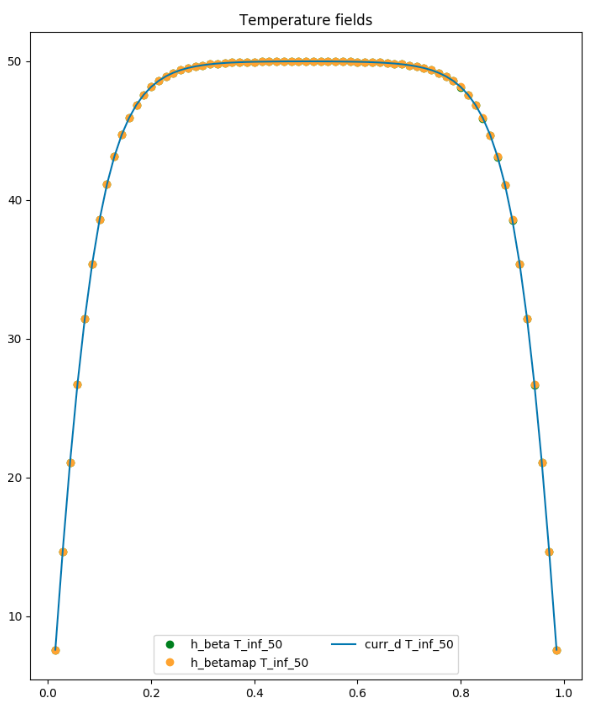
\includegraphics[height=10cm, width=8.43cm]{hbmap_50_VS_ObsField.png}
\caption{\small{\textbf{À gauche} : comparaison du champ $\bmap$ obtenu avec le code BFGS «maison» (points oranges) et du champ $\beta$ théorique obtenu à partir de \eqref{Ttrue}. Les points verts représentent un tirage de \eqref{distribbmap}. Les carrés mauves et noirs représentent les minimums et maximums des tirages (250) de $\beta$. \\ \textbf{À droite} : comparaison du champ de température exact, solution de \eqref{Ttrue} (ligne solide) avec la solution de \eqref{Tinex} en prenant $\bmap$ (points oranges) ou un tirage de \eqref{distribbmap} (points vert).}}
\label{comp_bmap_hbmap}
\end{figure}

\begin{figure}[!ht]
\centering
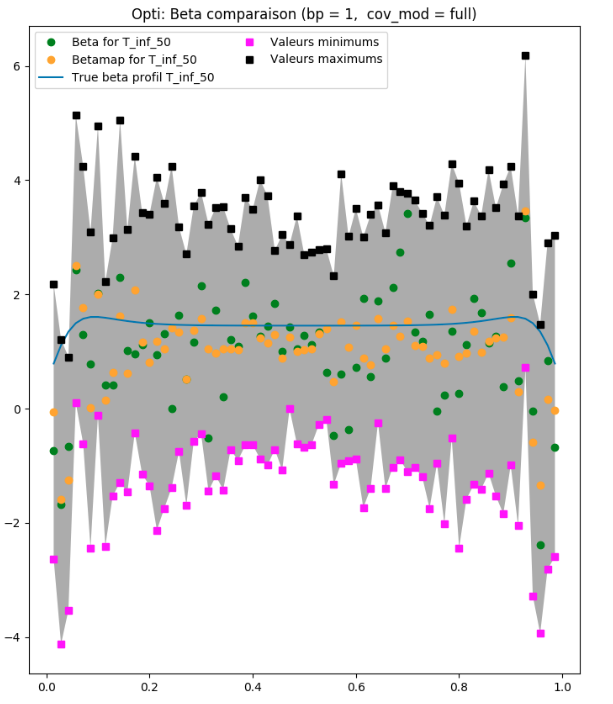
\includegraphics[height=10cm, width=8.43cm]{bmap_50_scipyVStheo.png} \hfill
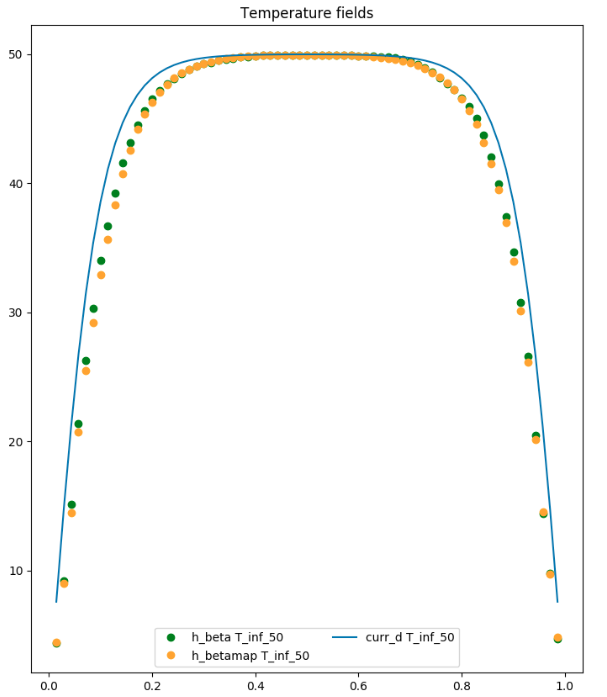
\includegraphics[height=10cm, width=8.43cm]{hbmap_50scipy_VS_ObsField.png}
\caption{\small{Même légende que Fig.\eqref{comp_bmap_hbmap}. La procédure est exactement la même que décrite précedemment sauf que le code BFGS utilisé est celui de Scipy. L'optimisation s'est vraisemblablement terminé avant convergence.}}
\label{scipycomp_bmap_hbmap}
\end{figure}

\dsb \subsubsection{Propagation d'une onde en fluide visqueux} \bk
\noindent L'équation de Burgers permet d'étudier la propagation des ondes et peut faire apparaître des chocs. Nous voulons dans un premier temps déterminer si l'inférence peut capturer les chocs. Dans un second temps, nous voulons déterminer si ce genre de méthode permet de capturer les non-linéarités. \\
Notons que cette démarche s'inscrit dans un projet plus vaste : utiliser une combinaison de méthode pilotée par les données et de machine learning pour construire un modèle de différences finies augmentées dépassant les capacités des méthodes de différences finies classiques.\\

\noindent Contrairement au cas précédent, l'équation de Burgers est instationnaire. Il a fallu alors écrire un code qui réalise une inférence à chaque itération temporelle. Le principe de l'inférence, la façon dont elle est réalisée et son objectif sont les mêmes que décrits plus haut.\\
\noindent L'équation de Burger visqueuse (VBE) s'écrit 
\begin{equation}
\frac{\partial u}{\partial t} + u \frac{\partial u}{\partial x} = \nu\frac{\partial^2 u}{\partial x^2}  \label{VBETrue} \tag{VBE}
\end{equation}
Nous résolvons cette équation en utilisant le schéma de Lax-Wendroff. La condition initiale est est un sinus de déphasage nulle, aniti-symétrique par rapport au centre du domaine.\\
Comme précédemment, il nous faut approximer cette équation avec un terme $\beta$ modélisant un des termes de l'équation précédente. \\
Nous remplaçons ici le terme non-linéaire de convection $\displaystyle u \frac{\partial u}{\partial x}$. On définit alors :
\begin{equation}
\frac{\partial u}{\partial t} + u \beta(x,t) = \nu \frac{\partial^2 u}{\partial x^2} \label{VBEbeta} \tag{VBE$\beta$}
\end{equation}
L'équation précédente est linéaire en $u$ alors que l'équation \eqref{VBETrue} ne l'est pas.\\
On définit la fonction de coût en comparant les solutions de ces deux équations. Si $n$ est l'itération courante, ajuster $\beta_n$ nécessite donc d'évaluer l'écart entre les solutions exactes et inexactes à l'itération $n+1$.\\
Pour éviter toute ambiguïté, on précise les indices dans la fonction de coût suivante 
\begin{equation}
\mathcal{J}^n = \frac{1}{2} \bepar{\bepar{U^{n+1}_{\text{obs}}}^\text{LW} - \bepar{U^{n+1}_\beta}^\text{CN}}^T \text{C}_\text{obs}^{-1} \bepar{\bepar{U^{n+1}_{\text{obs}}}^\text{LW} - \bepar{U^{n+1}_\beta}^\text{CN}} + \\ \lambda \bepar{\beta^n -
			\beta_{\text{p}}}^T \text{I}_d \bepar{\beta^n - \beta_\text{p}}
\end{equation}

\vspace{5mm}
\noindent De façon similaire au cas thermique, $\bmap^{n}$ sera obtenu en résolvant un problème d'optimisation :
\begin{equation}
\beta_{\text{MAP}}^n = \argmin \mathcal{J}^n
\end{equation}
Il est nécessaire de vérifier si les solutions sont similaires à toutes les itérations. Dans la figure Fig.\eqref{burger2it} une comparaison aux itérations 30 et 35 (sur 50) des champs $u^n_{\text{True}}$ et $u^n_{\beta}$ sont présentées. \\

\begin{figure}[!ht]
\vspace{-5mm}
\centering
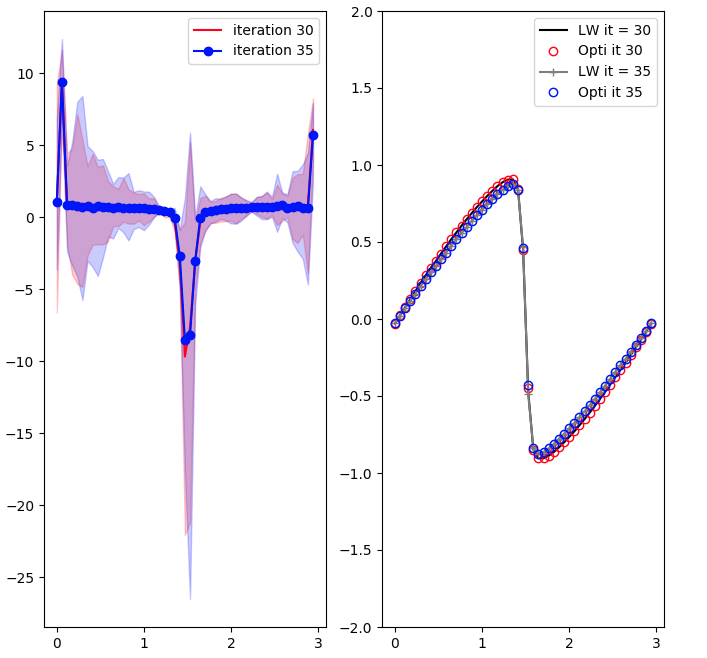
\includegraphics[scale=0.6]{burgers_deuxiteration35.png}
\caption{\small{\textbf{À droite}: comparaison des champs de vitesse exactes (lignes solides) et des $u\bepar{\bmap}$ (cercles) obtenues à partir de \eqref{VBEbeta}, des itérations \textit{temporelles} différentes. La correspondance est très précise. \textbf{À gauche} Les corrections $\beta$ et leurs variances, élevées à cause d'un nombre d'itération seuil fixé.}}
\label{burger2it}
\end{figure}
\noindent Sur la comparaison de gauche (Fig.\eqref{burger2it}) de gauche, les zones opaques représentent les variations possibles des distributions des $\bmap$. Leurs amplitudes assez grandes proviennent du fait qu'un nombre d'itérations maximales assez faible à été imposé lors de la minimisation.\\ 
Toujours est il que la superposition est parfaite pour toutes les itérations et qu'on a prouvé que l'inférence pouvait être utilisée même dans des cas instationnaires.\\
Le choc est bien capturé et la dissipation par effet visqueux dans la suite de la simulation est également parfaitement retrouvée.

\dsb \subsubsection{Effet dynamo et equations de Thomas 1d} \bk
\noindent Le cas turbulent de l'effet dynamo est un problème qui concerne la hausse ou le déclin d'un champ magnétique initialement faible, à l'intérieur d'un fluide conducteur, de turbulence développée (haut nombre de Reynolds).\\
Les équations de la Magnéto-Hydrodynamique (MHD) fournit les équations pour traiter de ce genre de problème. \cite{thomas1968numerical} établit des équations réduites pour traiter de ce problème, avec $u$ le champ de vitesse, $h$ le champ magnétique, et $\lambda$ la diffusivité magnétique : 
\begin{align}
\frac{\partial u}{\partial t} + u \frac{\partial u}{\partial x} -3h\, \frac{\partial h}{\partial x} &= \nu \frac{\partial^2 u}{\partial x^2} \label{uthomas} \\[3mm]
\frac{\partial h}{\partial t} + u \frac{\partial h}{\partial x} - h \frac{\partial u}{\partial x} &= \lambda \frac{\partial^2 h}{\partial x^2} 
\end{align}
Nous projetons de résoudre dans un premier temps en utilisant un solver de différence finie classique, avec un maillage très resséré pour être pris comme référence.\\
Puis nous injecterons un terme $\beta$ dans la première ou la deuxième (ou les deux) équations, utiliserons le procédé d'inférence pour reconstituer les champs $u$ et $h$.\\ On calculera les corrélations des deux champs après inférence mais également les spectres d'énergies afin de contrôler si la Physique est respectée.\\

\noindent Dans cette thèse, mettre en place une procédure d'inférence n'est pas une fin en soi, mais une étape qu'il était indispensable de maîtriser pour l'atteinte des objectifs visés.\\
Comprendre le formalisme mathématique de cet outil, avec la fonction de correspondance $\mathcal{L}$, l'optimisation de paramètres $\beta$ pour faire correspondre modèle et observations, permet d'avoir une première approche des algorithmes d'entraînement des intelligences artificielles comme le réseau de neurones.\\
En effet, les algorithmes de machine learning (ML) fonctionnent sur un principe très similaire à celui de l'inférence Bayesienne puisqu'ils cherchent à ajuster plusieurs paramètres (parfois des milliers voire des millions) afin de faire correspondre des entrées (\textit{inputs)} à des sorties, toutes les deux fournies par l'utilisateur; c'est ce qu'on appelle l'entraînement ou \textbf{\textit{training}}. Une fois ces paramètres établis, ces méthodes entendent prédire des sorties à partir d'entrées inédites, c'est ce qu'on appelle \textbf{la prédiction}.\\

\noindent L'idée de généraliser les données de l'inférence par ML est consiste en fait à découvrir la fonctionnelle liant les caractéristiques (\textit{inputs}) d'un problème et le vecteur $\bmap$ calculé au préalable sur plusieurs cas.\\
Avec la bonne architecture de réseau et des données assez variées, il devient possible d'utiliser le réseau comme une fonction qui à des entrées associe une sortie. Dans les cas qui nous occupe dans cette section, les entrées seront des grandeurs spécifiques au phénomère étudié, les sorties seront toujours des paramètres de correction.


\brick \subsection{Les réseaux de neurones} \bk 
\noindent Sans entrer dans trop de détails historiques ou mathématiques, le réseau de neurones (abrégé NN pour Neural Network) est un algorithme d'intelligence artificielle datant des années 50. Cette algorithme a été sous-estimé et sous-utilisé notamment parce que les ordinateurs de l'époque n'étaient pas en capacité d'exploiter les possibilités de cet outil et qu'on manquait de données.\\
Aujourd'hui les NN sont utilisés dans énormément de champs de la physique, de la médecine de l'informatique (évidemment) à tel point qu'ils sont omniprésents dans notre vie quotidienne. En ce qui concerne leur utilisation dans le domaine de la Turbulence, les NN se font de plus en plus de place. \\
On distingue deux grandes tendances dans l'utilisation des IA dans la turbulence : la première consiste à découvrir les \textit{équations} dans les données, on peut citer les travaux de \citep{kutz2017deep} ou \citep{raissi2018hidden} parmi beaucoup d'autres. \\
La deuxième approche, celle qui est suivie dans ce travail, est d'essayer de corriger les erreurs pour des modèles qui sont le plus utilisés, comme le \keps $ $. Les études de référence qui constituent la base de cette thèse sont \citep{parish2016paradigm}, \citep{singh2017machine}, \citep{wu2018data} ou encore \citep{wang2017physics} entre autres. \\

\noindent Cette approche peut faire émerger de nouveaux modèles, dits augmentées, qui pourraient ne pas être limités comme le sont les schémas aux différences finies. C'est l'idée qui se cache derrière l'injection du vecteur $\beta$ dans l'équation \eqref{VBEbeta}.\\
\noindent Nous allons revenir sur les cas évoqués lors de la section précédente et présenter la procédure de généralisation par NN.

\dsb\subsubsection{Présentation schématique d'un réseau de neurones} \bk
\noindent Schématiquement, un réseau de neurones est une succession de couches de \textit{neurones} densément liées par des poids $w$. Par analogie avec les neurones biologiques, les neurones dont il est question ici sont des éléments de l'algorithme qui somment toutes les entrées dans un sens, qui y ajoutent un biais (pour augmenter la généralisation) et qui transforment cette somme au travers une fonction non-linéaire dite $d'activation$. Par des algorithmes de \textit{backpropagation} les poids liant chaque couche sont ajustés pour minimiser l'écart entre la prédiction et la valeur de référence.
\begin{figure}[!ht]
\centering
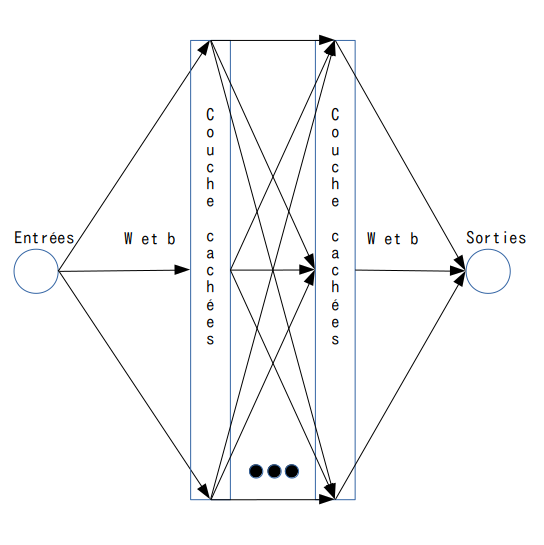
\includegraphics[scale=0.5]{NN_rapidoss.png}
\caption{\small{Représentation très schématique d'un réseau de neurones.}}
\label{NN_skeme}
\end{figure}
Les fonctions d'activations sont multiples et selon le problème (régression ou classification) l'une ou l'autre permettra une meilleure généralisation. Plusieurs articles comme \citep{krizhevsky2010convolutional} ont discuté des différentes fonction d'activations, et nous avons majoritairement utilisé la fonction SeLu :
\begin{equation}
\text{SeLu} = \lambda \,
\Big \{
		\begin{array}{c l}
		x & \text{if } x > 0 \\
		\alpha \bepar{ e^x - 1} & \text{if } x \leq 0
		\end{array}						
\end{equation}
Avec $\lambda$ et $\alpha$ ajustable, nous utilisons les valeurs de bases : $\lambda = 1\pnt 0507$ et $\alpha = 1 \pnt 6732$. Cette fonction d'activation possède des propriétés intéressantes dans le cadre du réseau de neurones que nous ne développerons pas ici \citep{klambauer2017self}.\\
Pour l'optimisation des poids, nous utilisons l'algorithme Adam \citep{kingma2014adam} qui minimise beaucoup plus vite la fonction de coût que le \textit{Gradient Descent} classique et qui devient le standard, du moins dans les problèmes de régression.\\

\dsb \subsubsection{Problème thermique} \bk
\noindent Jusqu'à présent, le problème inverse consistait à trouver $\beta$ en fonction des obervations. \\
La formulation du problème augmenté est directe, \cad  $ $, qu'on va chercher $\beta$ en fonctions de caractéristiques du problème.\\
La force de cette approche est que l'on peut choisir le nombres de caractéristiques que l'on veut, ou qui s'avèrent prodiguer la meilleur capacité de généralisation du réseau sur des problèmes inédits. L'optimisation des poids d'un NN amène à l'établissement de la fonctionnelle $\mathcal{F}$ : 
\begin{equation}
\beta = \mathcal{F}\bepar{\eta_1,\,\eta_2,\, ...,\eta_n}
\end{equation}
Les $\eta_i$ représentent les caractéristiques ou inputs choisies.\\
Dans le cas du problème thermique la température du fluide à l'extérieur du barreau \tinf $ $ ainsi que la température au point courant dans le barreau sont choisies comme $\eta_1$ et $\eta_2$. On cherchera alors donc : 
\begin{equation}
\beta_i = \mathcal{F}\bepar{T_{\text{inf}}, \, T_i}, \ \ \forall i \in \becro{0,\, N-1} 
\end{equation}
Il faut à présent contruire la matrice $X$ des entrées. Cette matrice prend la valeur du couple $\bepar{T_{\text{inf}}, \, T_i}$ pour tous les cas de \tinf $ $ considérés, et pour chaque point de discrétisation du domaine.\\
En face de ce couple, on fait correspondre la valeur de $\beta_i$ à laquelle on veut que nos poids et nos transformations nous amènent. La matrice des $\beta$ empilés sera notée $Y$.\\

\noindent On considère \tinf $ $ de 5 à 50 degré par pas de 5, soit 10 cas. L'espace est discrétisé en 69 points.\\
On découpe ensuite $X$ et $y$ en deux ensembles le \textit{training set} qui constitue 80 \% de $X$ et de $y$ et les 20 pourcents restant formeront le \textit{test set}. Les données seront préalablement aléatoirement mélangées pour briser toute corrélation entre les points.\\
Il faut également réduire et recentrer les données. On calculera la déviation standard et la moyenne sur le \textit{training set}; c'est l'échelle gardée pour la mise à l'échelle des nouvelles entrées pendant la phase de prédiction.\\

\noindent Comme pour l'inférence, on définit une fonction de coût qui compare $y_{\text{train}}$ avec les prédictions du réseau sur $X_{\text{train}}$ au fur et à mesure que les poids du NN sont ajustés. Par exemple, on peut construire la fonction de coût $\J$ des moindres carrées ordinaires (OLS) $y^*$ représentant la prédiction du réseau 
\begin{equation}
\J = \sum_{x, \, y\, \in\, \{X_{\text{train}},\, y_{\text{train}}\}} \bepar{y - y^*\bepar{x}}^2 \tag{OLS} \label{JOLS}
\end{equation}
On peut soit prendre la somme, soit prendre la moyenne de cet écart sur l'ensemble du training set. Nous avons utilisé cette fonction de coût mais également (et en majorité) la fonction de coût avec la régulariation sur la norme L1 des poids (Lasso):
\begin{equation}
\J = \sum_{x, \, y\, \in\, \{X_{\text{train}},\, y_{\text{train}}\}} \bepar{y - y^*\bepar{x}}^2 + \lambda \sum_{w\, \in\, W} |w| \tag{Lasso} \label{Lasso}
\end{equation}
On minimise cette erreur en cherchant la plus grande pente (voir les algorithmes de Gradient Descent \citep{Goodfellow-et-al-2016} ou Adam \citep{kingma2014adam}).\\
Enfin après avoir mis à jour les poids, on calcule $\J$ sur le test set. Si l'erreur est suffisamment basse, cela voudra dire que les poids du réseau sont optimum pour pouvoir généraliser les données de l'apprentissage.\\

\noindent On trace dans la figure Fig.\eqref{loglog_tempCost} l'évolution de la somme des erreurs sur le \textit{training set}. On évalue l'erreur sur le test set pour être sur de ne pas overfitté, on utilise le calcule de la valeur absolue de l'erreur moyenne\footnote{\url{http://scikit-learn.org/stable/modules/generated/sklearn.metrics.mean_absolute_error.html}} entre la prédiction de $X_{\text{test}}$ et $y_{\text{test}}$, elle est évaluée à $0 \pnt 011$.

\begin{figure}[!ht]
\centering
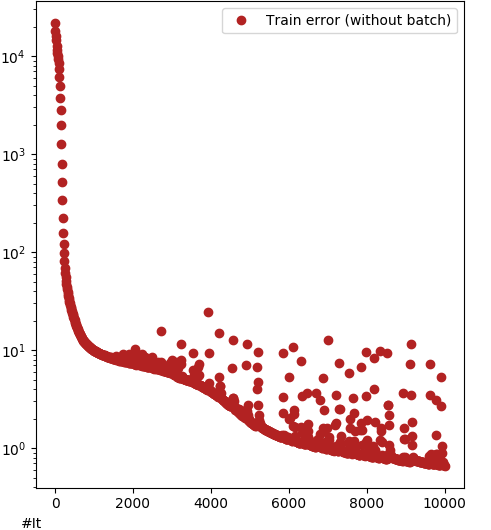
\includegraphics[scale=0.6]{loglog_Cost_ML_Temp.png}
\caption{\small{Évolution de \eqref{Lasso} évaluée sur le \textit{training set} au cours de l'optimisation des poids réseau. L'échelle est logarithmique.}}
\label{loglog_tempCost} \vspace{-3mm}
\end{figure}
\noindent L'entraînement s'est fait sur des cas dont la température extérieure \tinf $ $ est constante. Après s'être assuré que l'entraînement était efficace, nous avons testé l'algorithme pour prédire un vecteur de correction $\beta$ sur des cas différents. Nous présentons un cas avec $T_\infty =  35 - 15 \cos(\pi\,x)$.\\

\noindent Les prédictions sont faites sur $\beta$ puis on résout \eqref{Tinex} avec le $\beta$ prédit par le réseau de neurones. Comme nous l'avons précisé, nous nous assurons de la convergence du modèle en ajoutant un terme de dérivée temporelle pour pouvoir contrôler la convergence spatiale de la solution. \\
À chaque itération, le $\beta$ est prédit, puis la solution \eqref{Tinex} est calculée. Si le résidu entre deux itérations temporelles est inférieur à $10^{-7}$ la solution est considérée comme convergée.\\

\noindent On présente les prédictions du $\beta$ obtenu pour lequel le résidu est inférieur à la tolérance Fig.\eqref{beta35-15cospix}. Cette figure présente des zones où les $\beta$ prédits et théoriques sont bien différents. On pourrait s'attendre à une non-correspondance entre les champs de température prédit (solution de \eqref{Tinex}) et théorique (solution de \eqref{Ttrue}). Ces deux éléments sont représentés Fig.\eqref{Tbeta35-15cospix}.\\
Le fait que ces deux champs corroborent quasi-parfaitement dans l'ensemble du domaine peut s'expliquer par le fait que l'influence des termes linéaires modélisés par $\beta$ dans \eqref{Tinex} est faible por ce genre de température.\\
Cette intuition est vérifiée par l'incapacité du réseau de prédire une correction $\beta$ suffisante pour que la solution de \eqref{Tinex} soit précise pour des \tinf $ $  inférieurs ou égales à 15 degré. Pour palier à ce problème, on peut fournir plus de cas avec des \tinf $ $ dans cette plage et améliorer la prédiction des $\beta$ pour les cas intermédiaires.\\
\vspace{-0.3cm}
\begin{figure}[!ht]
\centering
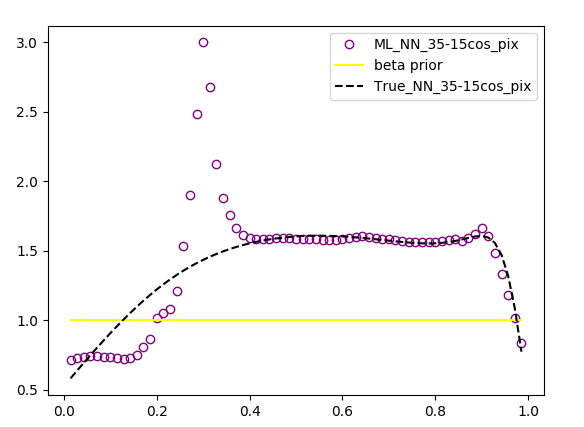
\includegraphics[scale=0.7]{Beta_NN_vs_True_35-15cos_pix.png}
\vspace{-3mm}
\caption{\small{Comparaison du $\beta$ théorique (pointillée) et des prédictions (cercles mauves). La ligne jaune symbolise le $\beta$ prior.}}
\label{beta35-15cospix}
\end{figure}

\begin{figure}[!ht]
\centering
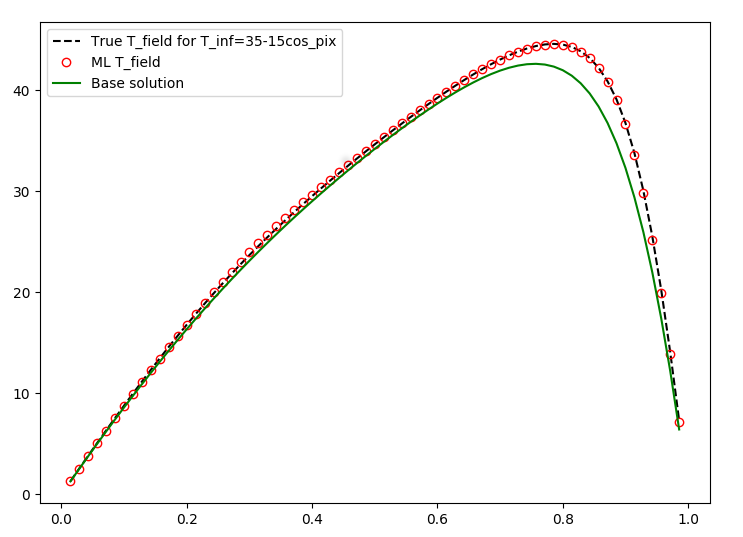
\includegraphics[scale=0.7]{T_True_vs_T_ML___T_inf_=_35-15cos_pix.png}
\vspace{-3mm}
\caption{\small{Comparaison du $T$ théorique (pointillée) et du T solution de \eqref{Tinex} avec $\beta$ présentés Fig.\eqref{beta35-15cospix} (cercles rouges). La ligne verte symbolise le champ de température T solution de \eqref{Tinex} avec $\beta$ prior.}}
\label{Tbeta35-15cospix}
\end{figure}

%\noindent On pourra schématiser un réseau de neurones comme une succession de transformations pour qu'un ensemble de données A (inputs) deviennent un ensemble B, de taille et composition différents.\\
%Les successions de transformation se font en couche et une matrice de poids lie chaque couche. \\
%L'idée du training d'un réseau de neurones et de trouver les poids qui maximisent la correspondance entre les entrées et les sorties.\\



%En parallèle, notre ère connait une hausse de l'utilisation d'algorithmes d'intelligence artificielle (IA) ou d'élaboration de procédés de résolution de problème pilotées par les données; et le nombre d'articles sur ces thèmes ainsi que leurs applications pratiques explosent. L'idée majeur de ce genre de méthode est le fait qu'on peut découvrir de l'information au sein des données afin de les généraliser (dans le cas d'IA.) ou de s'en servir pour corriger les prédictions de modèles peu fiables (dans le cas des méthodes pilotées par les données).\\
%Appliqués aux problématiques de la turbulence, ces algorithmes pourraient par exemple aider à identifier les régions ou les modélisations RANS ne sont pas fiables \citep{ling2015evaluation}, tirer le meilleure de résultats algébriques comme ceux de \citep{pope1975more} pour élaborer des modèles RANS augmentés par une IA type réseaux de neurones ou forêt aléatoire \citep{ling2016machine}.\\
%À partir de méthodes type inférence baysienne, on peut également construire des méthodes utilisant la structure de modèles RANS à une ou deux équations en injectant un vecteur de correction d'une itération à l'autre en comparant avec des cas dont les résultats DNS ou expérimentaux sont connus c'est en partie le travail effectué par \citep{singh2017machine}, \citep{parish2016paradigm} ou encore \citep{tracey2015machine} pour ne citer que quelques travaux.\\

%\href{./objectif.pdf}{This is my link}

\pagebreak

\dsb \subsubsection{Propagation d'une onde en fluide visqueux} \bk \label{burgerBIF}
\noindent On va ici utiliser les mêmes étapes que précédemment dans la construction de $X$ et $y$. Mais le choix des inputs est ici plus compliqué car le problème présente deux aspects à apprendre : 
\begin{itemize}[leftmargin=5mm]
\item[--] D'abord apprendre la fonctionnelle entre les entrées et les sorties;
\item[--] Et réfléchir pour prendre en compte la dynamique.
\end{itemize}   
Sur l'apprentissage de la dynamique beaucoup de travaux ont été effecutés notamment en utilisant des méthodes de réduction \citep{parish2016reduced}. Ces travaux se basent sur la théorie de \citep{chorin2002optimal} et \citep{tsung1995phase}. Ces méthodes sont en pleines expansions et nous projettons d'y passer encore du temps.\\

\noindent Sans utiliser ce genre de méthode, et sans se placer dans l'espace des phases, nous avons commencé à tester s'il était possible de résoudre l'équation de Brugers dans une forme linéaire avec un modèle de Crank-Nicholson augmenté par un NN.\\
Dans un premier temps, il faut réaliser l'inférence sur plusieurs cas en faisant varier la viscosité et en enregistrant la valeur du $\bmap$ pour tous les cas et toutes les itérations temporelles. \\
Il faut aussi veiller à ce que la valeur de la viscosité soit suffisamment élevée. Dans le cas contraire, les modèles numériques devenant instables au niveau du choc, des valeurs corrompues se propagent dans tout le domaine.\\

\noindent Il a fallu alors réfléchir aux inputs $\eta_i^n$ à choisir pour constituer la fonctionnelle $\beta^n = \mathcal{F}\bepar{\eta_i^n}$ . En s'inspirant des différence finies, nous avons considéré un nœud spatial centré au point $i$ de l'itération $n$ : $$X = \{ u^n_{i-1},\, u^n_{i},\, u^n_{i+1}\}$$. L'idée est de déterminer si il était possible de trouver dans les données une corrélation spatiale propre au champ de vitesse.\\
Nous avons également essayé de rajouter les coordonnées spatiales dans chacun des entrées, améliorant la réduction de l'erreur sur le \textit{training set}. La matrice d'entrées devint alors $$X = \{ x_{i-1}, \, x_i,\, x_{i+1},, u^n_{i-1},\, u^n_{i},\, u^n_{i+1}\}$$
Enfin nous avons également considéré des entrées prenant les valeurs du champ de vitesse aux itérations précédentes (une ou deux). Nous écrivons la matrice $X$ pour une itération : $$ \beta^{n+1} = \bepar{x_{i-1}^n, x_i^n, x^n_{i+1}, U_{_{\bk i-1}}^{\red n-1}, U_{\bk i}^{\red n-1}, U_{_{\bk i+1}}^{\red n-1}, U_{i-1}^n, U_i^n, U^n_{i+1}} $$\\
Tout ces cas sont encore en cours de traîtement, en effet la majeur contrepartie dans ce problème est le manque de diversité de données sur lesquelles les inférences ont été effectuées. Les résultats n'étaient pas probants, il fut long de comprendre la source des erreurs. \\
Dans la suite de la thèse, nous investiguerons ces différents cas et tenterons de déterminer lequel de ces modèles fournira des résultats les plus physiquement viables.\\
En parallèle nous avons eu l'idée de développer un solver en utilisant directement le réseau de neurones, sans passer par une phase d'inversion.\\

\dsb \subsubsection{Aller Plus loin} \bk
\noindent De nombreux codes effectifs ont été écrits au cours de cette première année et de nombreuses idées ont été élaborées. Puisqu'il fallait d'abord mettre l'accès sur les objectifs premiers de la thèse, certain ont été mis temporairement de côté.\\
 Néanmoins, il est possible qu'au cours des deux prochaines années, certaines d'entre elles reviennent au centre de nos travaux.
 \begin{itemize}[leftmargin=1cm]
 \item[--] Problème de MHD : retrouver par inférence le champ magnétique de la Terre à l'intérieur des données DNS pour améliorer les solver moins coûteux, et mieux connaître ce champ;
 \item[--] Proposer un modèle de EDQNM pouvant traiter des cas de turbulence inhomogène ou anisotrope en inférant un terme instationnaire à partir de données DNS;
 \item[--] Faire du tracking de structures turbulentes pour étudier directement l'évolution d'une instabilité, explorer pourquoi pas les régimes de transitions.
 \end{itemize}

\noindent Nous avons également tenté d'utiliser les réseaux de neurones comme force brute pour prédire la physique, sans passer par une phase d'inférence qui peut s'avérer assez longue.
\navy \section{Utiliser les IA pour prédire la physique} \bk \label{NNdirect}
\noindent Cette partie est une ébauche de deux travaux en cours. Nous allons tout d'abord présenter les premiers résultats sur l'utilisation d'un réseau de neurones pour la prédiction d'une solution de l'équation de Burgers, y expliquer la procédure que nous avons suivi et également les éléments que nous cherchons à améliorer. \\
Nous parlerons alors d'un aspect fondamental des NN : leur architecture.\\
La deuxième partie traitera de l'apprentissage renforcée. Nous y consacrerons quelques lignes car l'idée est encore naissante.
\brick \subsection{Propagation d'ondes en milieu visqueux}\bk
\noindent Nous reprenons notre équation de Burgers visqueux monodimensionnel : 
\begin{equation}
\frac{\partial u}{\partial t} + u \frac{\partial u}{\partial x} = \nu\frac{\partial^2 u}{\partial x^2}  \label{VBETrue2} \tag{VBE}
\end{equation}
L'idée ici n'est plus d'injecter un terme à découvrir mais de générer des solutions de cette équations pour des conditions initiales sinusoïdales différentes et tenter d'apprendre à un NN la dynamique régie par \eqref{VBETrue2}. On représente les différentes conditions initiales dans la figure Fig.\eqref{initNN}

\begin{figure}[!ht]
\centering
\vspace{-5mm}
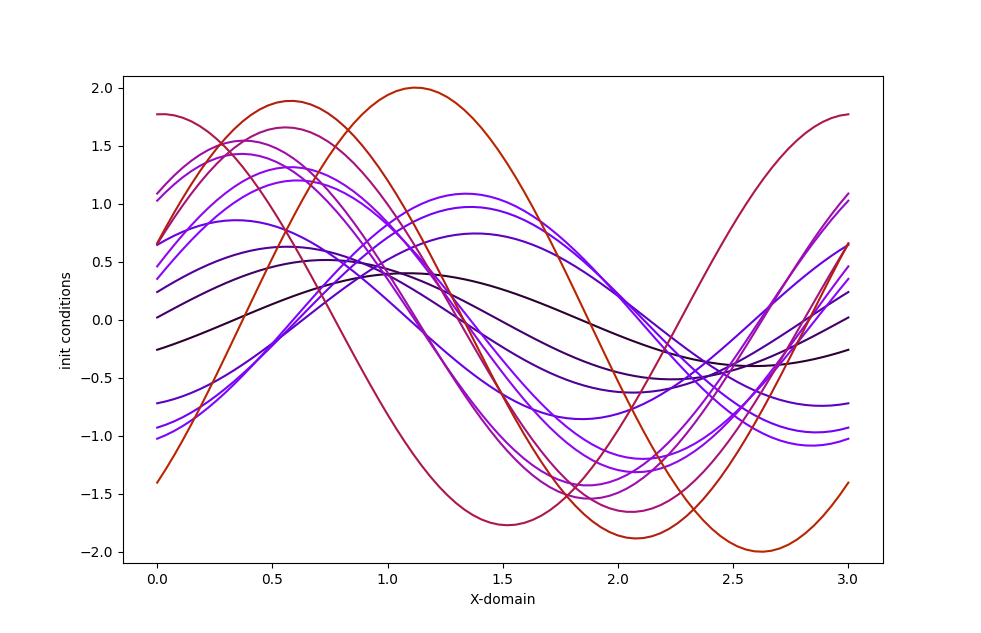
\includegraphics[scale=0.6]{Initialisation_cases.png}
\caption{\small{Différentes conditions intiales résolues avec un solver Lax Wendrof sur 80 itérations temporelles. Les solutions à toutes les itérations sont utilisées pour entraîner un réseau de neurones.}}
\label{initNN}
\end{figure}

\noindent Avec un solver Lax-Wendroff, nous résolvons sur 80 itérations temporelles les différentes conditions initiales et enregistrons les champs de vitesse pour chacune des itérations.\\
Puis nous voulons construire les matrice $X$ et $y$. Comme nous l'avions évoqués dans le paragraphe \eqref{burgerBIF}, cette étape est délicate car il existe une infinité de possibilités. Ici nous avons considéré des lignes d'entrées telles que :
\begin{multicols}{2}
	\noindent
	$$ X = \left[ \begin{array}{c} \cdot \\ U^n_{i-1},U^n_{i}, U^n_{i+1}, \frac{U^n_{i+1} - U^n_{i-1}}{2\Delta x}  \\ \cdot 
					  \end{array}
		   \right]
	$$
	\columnbreak
	$$ y = \left[ \begin{array}{c} \cdot \\ U^{n+1}_i \\ \cdot 
			  \end{array}
	   \right]
	$$
	\end{multicols}
  
\noindent Avec $U_i^n$ la valeur de la vitesse au i$^{\text{ème}}$ point de discrétisation spatiale, à la n$^{\text{ème}}$ itération temporelle.\\
 Les trois premiers inputs imitent les schémas aux différences finies classique avec une maille centré, la quatrième caractéristiques est le taux de variations de ce champ de vitesse pour renseigner la valeur de la pente sur à chaque point \footnote{Cette dernière entrée a été rajoutée après avoir constaté que des informations étaient nécessaire au NN pour découvrir la fonctionnelle}. \\
 Finalement la fonctionnelle $\mathcal{F}$ s'écrit $$U^{n+1}_i =  \mathcal{F}\bepar{U^n_{i-1},U^n_{i}, U^n_{i+1}, \frac{U^n_{i+1} - U^n_{i-1}}{2\Delta x}}$$.\\
   On découpe $X$ et $y$ en un \textit{training set} et une partie de nos données pour tester le \textit{training}, nous recentrons les données conformément à ce qu'lon a évoqué plus tôt, et commençons l'optimisation des poids avec la fonction d'activation SeLu pour l'ensemble des neurones et l'algorithme Adam pour l'optimisation. L'architecture du réseau est la suivante : 6 couches de 80 neurones.\\
    On représente la fonction de coût figure Fig.\eqref{trainingNNvbe}
    \begin{figure}[!ht]
    \centering
    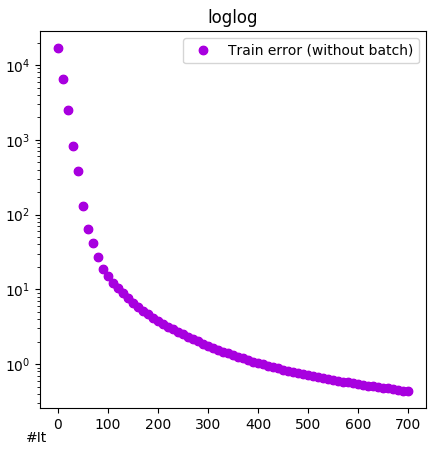
\includegraphics[scale=0.6]{loglogvbeNN.png}
    \caption{\small{Evolution de la fonction de coût \eqref{Lasso}} pour la prédiction de la physique directe. La courbe tracée n'est pas la moyenne des erreurs mais la sommes des erreurs commises sur les prédiction sur tout $X_{\text{train}}$ }
    \label{trainingNNvbe}
    \end{figure}
    
\noindent Le choix de l'architecture est fortuit. Nous avions écrit un algorithme génétique pour découvrir l'architecture optimale en revanche ce sont des algorithmes qui nécessitent énormément de temps; nous l'avons donc pas encore utilisé sur ce cas.\\
L'erreur de la fonction de coût décroît fortement jusqu'à quelques unités. Nous n'avons pas augmenté le nombre d'itération pour ne pas avoir à faire aux problèmes liés à l'overfitting.\\

\noindent Nous générons à présent une condition intiale nouvelle par rapport aux $X$  et $y$. Nous comparons les prédictions à chaque itération avec les données exactes obtenues en résolvant cette condition intiale dans le solver LW. \\
\begin{figure}[!ht]
\centering
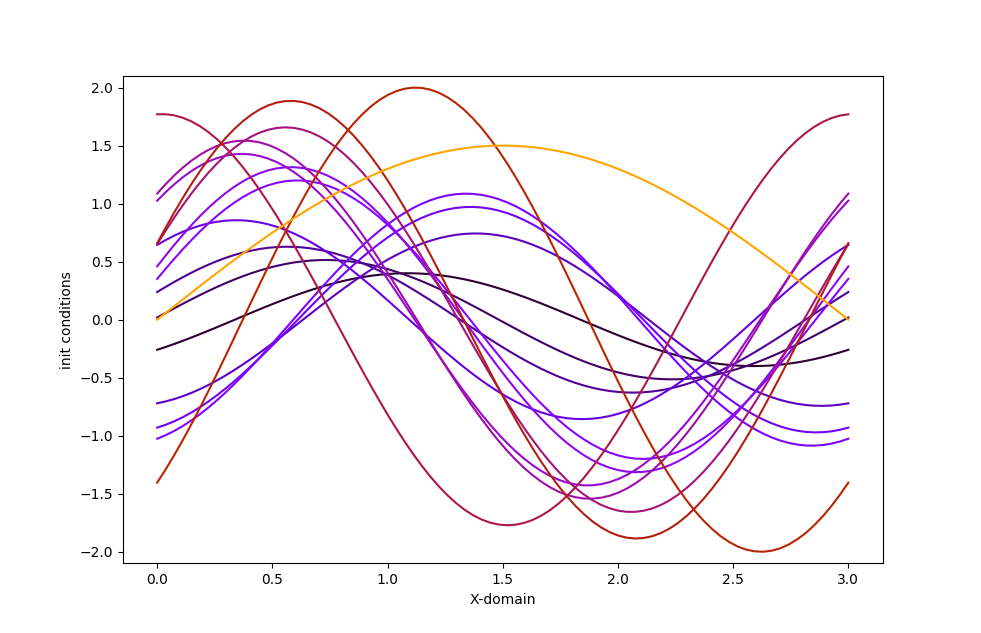
\includegraphics[scale=0.5]{Initialisation_cases_Andu1.png}
\caption{\small{Nous voulons prédire l'évolution du champ de vitesse orange différent en amplitude et déphasage des données utilisées pour l'entraînement}}
\label{newinputNN}
\end{figure}

\noindent Les figures qui suivent présentent les comparaisons (partie inférieure), les erreurs relatives (partie supérieure gauche) et la norme infinie de l'erreur (partie supérieure droite).

\begin{figure}[!ht]
	\centering
	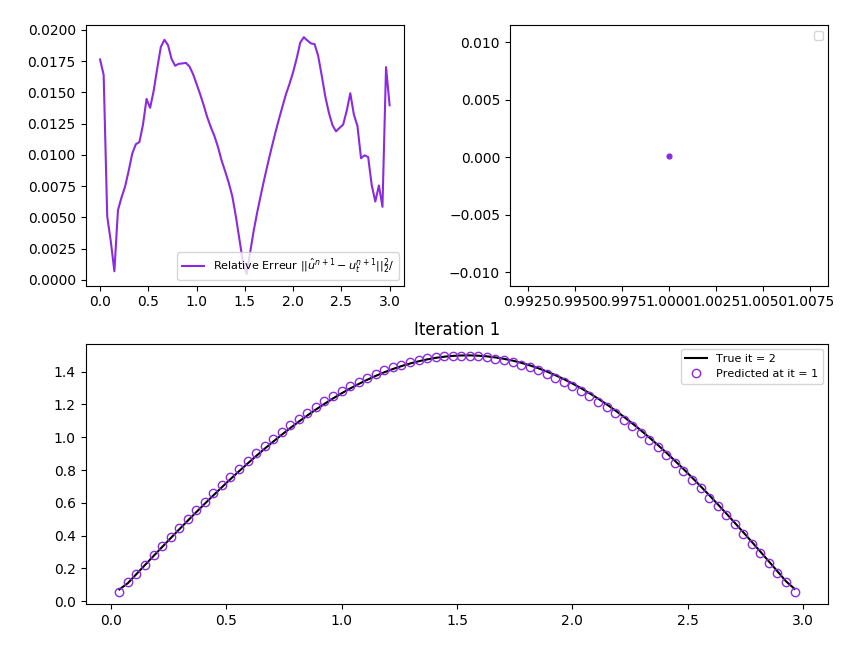
\includegraphics[scale=0.6]{Pres_First_Iteration_1.png}
	\caption{\small{Comparaison entre la deuxième itération du LW et la prédiction du NN utilisant le champ de la première itération comme unique référence.}}
	\label{FirstItNewNN1}
\end{figure} 

\pagebreak

\begin{figure}[!ht]
	\centering
	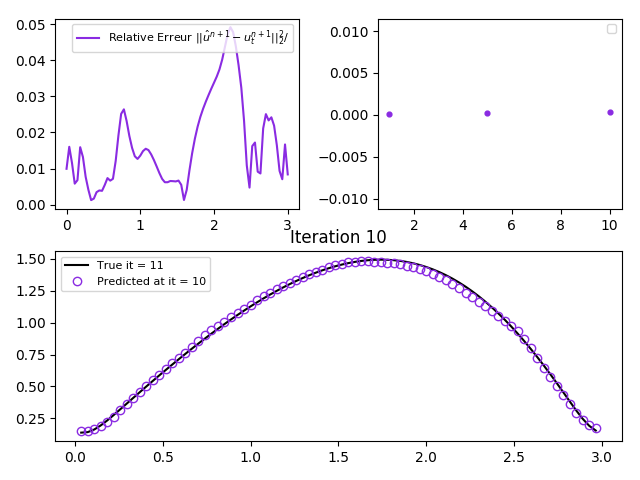
\includegraphics[scale=0.75]{Pres_Tenth_Iteration_1.png}
	\caption{\small{Comparaison entre la onzième itération du LW et la prédiction du NN utilisant le champ de la dixième itération comme unique référence.}}
	\label{10ItNewNN1}
\end{figure} 

\begin{figure}[!ht]
	\centering
	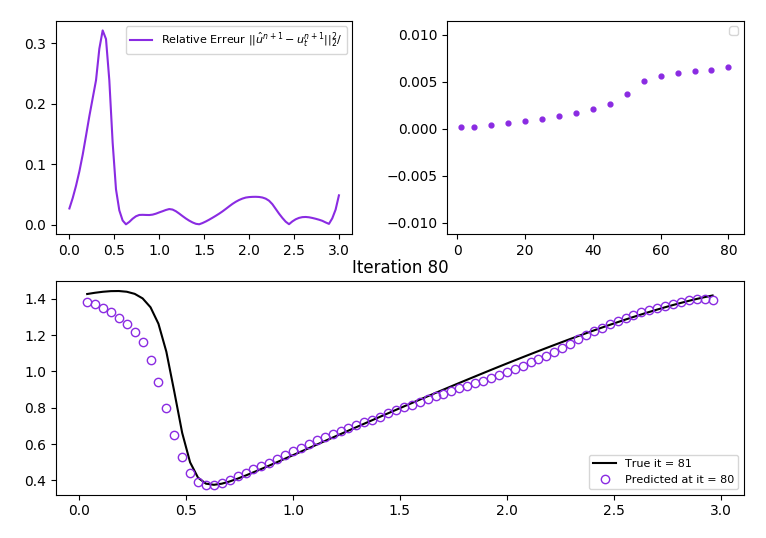
\includegraphics[scale=0.67]{Pres_Last_Iteration_1.png}
	\caption{\small{Comparaison entre la 81 ème itération du LW et la prédiction du NN utilisant le champ de la 80 ème itération comme unique référence.}}
	\label{LastItNewNN1}
\end{figure}


\noindent Au fur et à mesure que les itérations se déroulent, les erreurs sur les prédictions s'accumulent corrompant petit à petit les entrées des NN. Cela met en évidence deux origines d'erreur : une locale propre à chaque prédiction, et une globale qui s'accumule.\\
Nous avons testé d'autres cas pour lesquels les erreurs n'étaient pas si grandes mais le cas présenté représente bien la question : comment contrôler l'erreur global ?\\
La première solution proposé est de modifier la fonction de coût en prenant en compte dans la minimisation la variation des sorties en fonction des entrées \citep{pan2018long}. Des résultats avec cette méthode n'ont pas été probant dans notre cas, nous avons décidé de nous concentrer sur une méthode plus efficace mais également en complète expansion : l'apprentissage renforcé ou \textit{reinforcement learning}.

\brick \subsection{Le reinforcement learning (RL)} \bk \label{sec_REIL}
\noindent Le RL est une partie des machine learning dans lequel un agent apprend à se comporter dans un environnement en réalisant des «actions» selon une politique qui donne des critiques positives ou négatives.\\
L'agent exécute des actions; si on prend l'exemple du jeu pac-man, l'agent est le pac-man. Il peut aller dans quatre directions (haut, bas, droite, gauche). \\
La politique sera "critique neutre  tant que pac-man avance", "critique positive si pac-man mange des pac-gommes" et : "critique négaive sur les fantômes mangent par-man".\\
La prise de décision se fait en analysant l'environnement. Dans le cas du pac-man l'environnement est une série d'images où les fantômes, les pac-gommes et le pac-man sont identifiés.\\
 Ainsi le RL peut se résumer dans la boucle suivante : 
\begin{figure}[!ht]
 \centering
 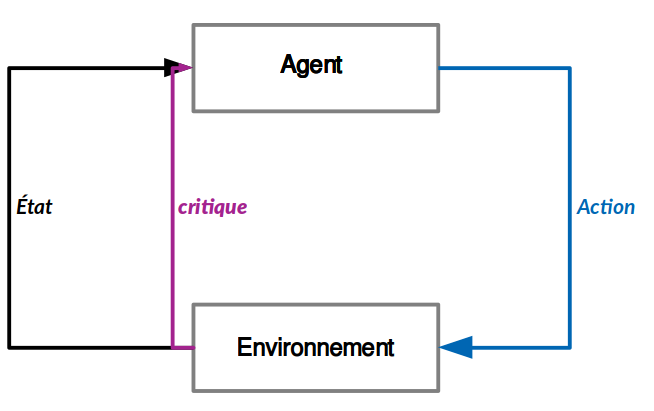
\includegraphics[scale=0.5]{RL_scheme.png}
 \caption{\small{Schéma classique représentant les actions et rétroactions des agents et de l'environnement dans le cas de l'apprentissage renforcé.}}
 \label{boucleRL}
 \end{figure} 
 
 \noindent D'un point de vue plus mathématique, pour être sur que l'agent apprennent bien de l'environnement, il faut parcourir l'ensemble des états ET l'ensemble des actions pour pondérer sa prise de décision. Ces différentes étapes sont toutes comprises dans l'équation de Bellman sur laquelle est basée le RL. En résolvant cette équation, on trouve la politique qui permet de prendre les meilleures actions. \\
La résolution de cette équations nécessite une exploration de toutes les actiones possibles pour les différents états et leur devenir. C'est pourquoi cette méthode peut nécessiter beaucoup de temps. \\

\noindent Très récemment, l'idée de considérer un NN comme agent est née. C'est ce qu'on appelle le\textit{Deep Reinforcement Learning} (DRL). Le réseau est entraîné au fur et à mesure que les états sont explorés. Les actions sont ici toujours les mêmes puisqu'il s'agit d'effectuer une prédiction à travers un NN, mais les poids de ce NN seront modifiés au fur et à mesure selon la critique. On appelle ce genre d'algorithme des \textbf{\textit{actor-critics}}.
\noindent Pour l'instant l'ensemble de la littérature sur ce sujet considère des \textit{images} comme environnement. Nous essayons en ce moment d'élaborer un algorithme considérant des critiques liées à la physique comme la conservation de l'énergie.

\pagebreak

\navy \section{Conclusion} \bk
\noindent Pour résumer, nous nous sommes tout d'abord concentrés sur les basiques du ML et sur les articles de références comme ceux cités dans le corps du rapport. Ces premiers pas nous ont permis de nous familiariser avec les mathématiques propres à la discipline et nous a aidé à mieux comprendre les enjeux des méthodes et du projet.\\
À partir d'une étude bibliographique, nous avons pu déterminer les pistes à approfondir pour tenter de mener à bien notre projet et d'utiliser toute la puissance des IA tout en étant sur que les prédictions sont précises et fiables physiquement.\\
Nous avons alors commencé à explorer plusieurs méthodes : des méthodes à deux temps comme la combinaison inférence/Machine learning (section \eqref{combiNN_inference}) ou bien des méthodes de prédiction directes (section \eqref{NNdirect}). \\
Nous avons également cherché à aller au delà des équations de Burgers ou que des cas thermiques, comme les modèles de MHD les plus utilisés.\\
	
\noindent Comme évoqué dans le paragraphe \eqref{sec_REIL}, nous étudions la possibilité d'utiliser les algorithmes d'apprentissage renforcé profond (DRL) pour imposer une direction d'apprentissage vers la bonne solution dans le sens de la Physique.\\
Nous espérons pouvoir ensuite comparer qualitativement et quantitativement les solutions issus des DRL, des NN et des combinaisons ML/inférence.\\





\pagebreak

\bibliographystyle{apalike}
\bibliography{bibliotheque}


\end{document}